\documentclass[main.tex]{subfiles}

\begin{document}
\newcommand{\Y}{\mathcal{Y}}
\newcommand{\X}{\mathcal{X}}
\section{Introduction}

\begin{defin}
  \begin{itemize}
  \item La \emph{quantification} est une génération non réversible qui permet à
    une source $X$ à valeur dans $\X$ d'associer un index $I\in\{0,...M-1\}$ ou
    $M$ est le nombre de cellule de quantification. La
  \item \emph{quantification inverse} consiste à associer une estimée $\hat{X}$ de $X$ à valeur dans $\X$ à un index $I$.
  \item
Pour cela on introduit une fonction de quantification :

\[
  q :\X \to \{0,...,M-1\}
\]
et des fonction de quantification inverse:
\[
  r :\{0,...,M-1\} \to \X
\]
\item Pour une réalisation $x$ de $\X$,$i = q(x)$ est l'index de quantification.
  \[
    \hat{x}= r(q(x)) = Q(x)
  \]
  est la valeur reconstruite/quantifiée.
  \end{itemize}
\end{defin}
\begin{rem}
  Si $\X = \N $ ou $\Z$ ou $\R$ on réalise une quantification vectorielle. Si $\X =\R^n$ on réalise une quantification vectorielle.
\end{rem}

Les quantifications sont optimisées de manière à obtenir un débit minimale sous contrainte de distortion ou bien une distortion minimale sous contrainte de débit. La distorsion étant une mesure de l'erreur entre $X$ et $\hat{X}$.

Un quantificateur est défini par des intervalles de quantification $b_0 < b_1 < ... < b_n$ et par des valeurs de reconstitution $y_1,...,y_n$ : si on a $x \in[b_{i-1} ; b_i[$ alors $Q(x) = y_i$.
Dans la suite, on va voir comment régler de façon efficace les $b_i$ et les $y_i$.
\section{Distorsion et mesure de distorsion}
\begin{defin}

  On introduit une mesure de distorsion pour les performances d'un quantificateur qui toute les bonnes propriétés d'une distance symétrique, définie positive). Les principales mesures considérées sont:
  \begin{itemize}
  \item la mesure de distorsion en valeur absolue, $d(x,y) = |x-y|$
  \item la mesure de distorsion quadratique, $d(x,y) = (x-y)^2$
  \item le mesure de distorsion de Hamming, $d(x,y) =
    \begin{cases}
      0 & \text{ si } x=y \\
      1 & \text{ sinon}
    \end{cases}$
  \end{itemize}
\end{defin}

Pour une source $X$ décrite par une distribution de probabilité $f_X(x)$, la distorsion introduite par un quantificateur $Q(x)$, est la moyenne de la mesure de la distorsion:
\[D = \int_{-\infty}^{\infty} d(x,Q(x))f_X(x) dx  = E(d(X,Y))\]
Pour la mesure de distorsion quadratique, on a:
\[D = \int_{-\infty}^{\infty} (x-Q(x))^2f_X(x) dx \]

\section{Quantification scalaire}
\subsection{Quantification uniforme d'une source uniforme}

On considère une source $X$ uniformément distribuée sur $[-X_{max} ; X_{max}]$. On considère aussi un quantificateur uniforme, c'est à dire que les intervalles de quantification sont tous de même taille, à M niveaux de sortie, situés au milieux des intervalles de quantification.
Prenons par exemple, un quantificateur à 4 niveaux de quantification:
%\img{0.5}{2/1/2.png}
\begin{center}
  \begin{tikzpicture}
    \begin{axis}
      [axis lines =middle,
      xmin=-3,xmax=3,
      ymin=-2,ymax=2,
      xtick={-2,-1,1,2},
      ytick={0.5,1.5},
      xticklabels={$-X_m$,$-\frac{X_m}{2}$,$\frac{X_m}{2}$,$X_m$},
      yticklabels={$\frac{X_m}{4}$,$\frac{3X_m}{4}$},
      ]
      \addplot[black] plot coordinates {(-2,-1.5) (-1,-1.5)};
      \addplot[black] plot coordinates {(-1,-0.5) (0,-0.5)};
      \addplot[black] plot coordinates {(0,0.5) (1,0.5)};
      \addplot[black] plot coordinates {(1,1.5) (2,1.5)};

      \addplot[black,dashed] plot coordinates {(-1,-1.5) (-1,-0.5)};
      \addplot[black,dashed] plot coordinates {(1,0.5) (1,1.5)};
    \end{axis}
  \end{tikzpicture}%
  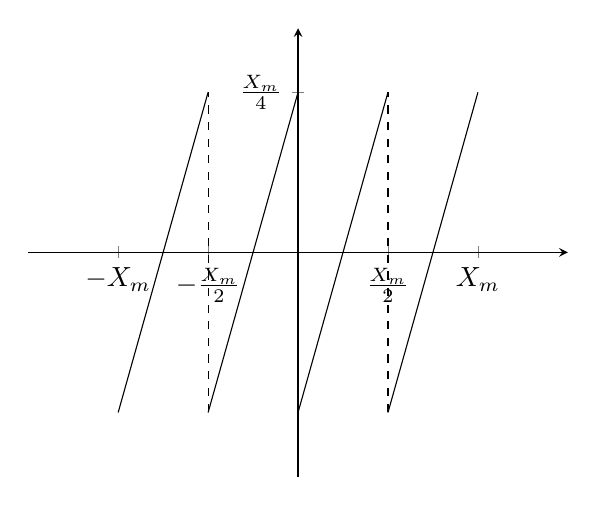
\begin{tikzpicture}
    \begin{axis}
      [axis lines =middle,
      xmin=-3,xmax=3,
      ymin=-0.7,ymax=0.7,
      xtick={-2,-1,1,2},
      ytick={0.5},
      xticklabels={$-X_m$,$-\frac{X_m}{2}$,$\frac{X_m}{2}$,$X_m$},
      yticklabels={$\frac{X_m}{4}$},
      ]
      \addplot[black] plot coordinates {(-2,-0.5) (-1,0.5)};
      \addplot[black] plot coordinates {(-1,-0.5) (0,0.5)};
      \addplot[black] plot coordinates {(0,-0.5) (1,0.5)};
      \addplot[black] plot coordinates {(1,-0.5) (2,0.5)};
      \addplot[black,dashed] plot coordinates {(-1,-0.5) (-1,0.5)};
      \addplot[black,dashed] plot coordinates {(1,-0.5) (1,0.5)};

    \end{axis}
  \end{tikzpicture}
\end{center}
On note $\Delta$ l'intervalle de quantification, dans ce cas, $\Delta = \frac{2 X_{max}}{M}$.\\

Pour déterminer la distorsion qui va être introduite par le quantificateur, on calcule simplement:

\begin{align*}
D &= \int_{-X_{max}}^{X_{max}}\frac{1}{2X_{max}}(x-Q(x))^2 dx
\intertext{Comme $Q(x)$ est connu et constant sur un intervalle de quantification, on découpe simplement l'intervalle en sous-intervalles de quantification:}
D &= \sum_{i=0}^{(M-1)} \int_{i\Delta}^{(i+1)\Delta} \frac{1}{2X_{max}}(x-(i+\frac{1}{2})\Delta)^2 dx
\intertext{On calcule}
    I & = \int_{i\Delta}^{(i+1)\Delta} (x-(i+\frac{1}{2})\Delta)^2  \frac{1}{2X_{max}} dx \\
  \intertext{on pose $u = x+X_{max}-(x+\frac{1}{2})\Delta)$}
& = \int_{-\Delta/2}^{\Delta/2} \frac{u^2}{2X_{max}} du \\
I & = \frac{\Delta^3}{24X_{max}} = \frac{X_{max}^2}{3M^3}
\end{align*}

Dans $D$, on a $M$ intégrales égales à $I$ donc \[ D = \frac{X_{max}^2}{3M^2}\]

L'énergie de la source est mesurée par sa variance
\begin{align*}
\sigma^2 & = \int_{-\infty}^{+\infty} x^2 f(x) dx \\
& = \int_{-X_{max}}^{X_{max}} \frac{x^2}{2X_{max}} dx \\
\sigma^2 & = \frac{X_{max}^2}{3}
\end{align*}

On obtient donc $D = \frac{\sigma^2}{M^2}$.
\begin{prop}
Sans codage entropique, le nombre de bits nécessaires pour représenter un niveau de reconstruction est $R = \lceil \log_2 M \rceil $, d'où
\[ \boxed{ D = \sigma^2 2^{-2R} } \]

\end{prop}
La distorsion maximale est égale à l'énergie de la source, et diminue très rapidement quand on augmente le nombre de bits du quantificateur.

\begin{rem}
Dans certains cas (source non uniforme), un codage entropique peut permettre de réduire le débit.
\end{rem}

Rapport signal à bruit :
\begin{align*}
RSB & = \frac{\sigma^2}{D} = 2^{2R} \\
RSB_{dB} & = 10\log_{10}(2^{2R}) = 6.02R \text{decibel}
\end{align*}

Le $RSB$ est utilisé comme mesure de qualité en audio, image...

\begin{center}
  \begin{tikzpicture}
    \begin{axis}
      [axis lines = middle,
      xmin=0,xmax=5,ymin = 0,ymax=8,
      xlabel=$R$(bits),
      ylabel=$\sigma_x^2$,
      ytick={0.5,2,8},
      yticklabels={$D/16$,$D/4$,$D$},
      ]
      \addplot[red,mark=+,samples at={0,1,2,3,4,5}] {2^(-2*(x-1.5)};
      \addplot[gray, dashed,no marks,xcomb,samples at={0,1,2,3,4,5}] {2^(-2*(x-1.5)};

    \end{axis}
  \end{tikzpicture}
\end{center}
La pente a l'origine est de $-2\ln(2)\sigma_x^2$. La distorsion décroit très vite avec $R$

On peux aussi tracer la courbe distortion- débit (R= f(D))


\subsection{Quantification uniforme d'une source quelconque}

On considère une source $X$ décrite par sa ddp $f_X(x)$, quantifiée par un quantificateur uniforme à $M$ niveaux de pas $\Delta$. Si $M$ est fini on peux considérer deux type de quantificateur:

\paragraph{Exercice}
  \begin{enumerate}
  \item Générer N réalisation d'une source Gaussienne $\mathcal{N}(0,1)$.
  \item Implanter un quantificateur uniforme sans zone morte et la fonction de reconstruction associée.
  \item Faire de Meme pour un quantificateur avec zone morte.
  \item Tracer dans les deux cas la courbe débit distorsion en supposant que les index de quantification sont codées à l'aide d'un codeur entropique.
  \end{enumerate}


\begin{figure}[H]
  \centering
  \begin{subfigure}{0.5\textwidth}
  \begin{tikzpicture}
    \begin{axis}
      [axis lines =middle,
      xmin=-3,xmax=3,
      ymin=-3,ymax=3,
      xtick={-2,-1,1,2},
      ytick={-1.5,-0.5,0.5,1.5},
      xticklabels={$-2\Delta$,$-\Delta$,$\Delta$,$2\Delta$},
      yticklabels={$\frac{-3\Delta}{2}$,$\frac{-\Delta}{2}$,$\frac{\Delta}{2}$,$\frac{3\Delta}{2}$},
      x tick label style={font=\tiny},
      y tick label style={font=\tiny,anchor=center,xshift=-(sign(\ticknum-1.5))*1em},
      ]
      \addplot[black, jump mark left,thick]coordinates {(-2,-1.5)
        %(-1,-1.5)
      (-1,-0.5)
      (0,0.5)
      (1,1.5) (2,1.5)};
    \end{axis}
  \end{tikzpicture}
  \subcaption{Quantificateur sans zone morte}
\end{subfigure}%
  \begin{subfigure}{0.5\textwidth}
  \begin{tikzpicture}
    \begin{axis}
      [axis lines =middle,
      xmin=-3,xmax=3,
      ymin=-3,ymax=3,
      xtick={-3,-2,-1,1,2,3},
      ytick={-2.5,-1.5,1.5,2.5},
      xticklabels={$-d-2\Delta$,$-d-\Delta$,$-d$,$d$,$d+\Delta$,$d+2\Delta$},
      yticklabels={$-d-\frac{3\Delta}{2}$,$-d-\frac{\Delta}{2}$,$d+\frac{\Delta}{2}$,$d+\frac{3\Delta}{2}$},
      x tick label style={font=\tiny},
      y tick label style={anchor=center,font=\tiny,xshift=-(sign(\ticknum-1.5))*2em}]
      \addplot[black,thick, jump mark left]coordinates {(-3,-2.5)
        %(-1,-1.5)
        (-2,-1.5)
        (-1,0)
      (1,1.5)
      (2,2.5)
      (3,2.5)};
    \end{axis}
  \end{tikzpicture}
  \subcaption{Quantificateur avec zone morte}
\end{subfigure}
\end{figure}


On considère une source $X$ discrète décrite par une ddp $f_X(x)$. On cherche le quantificateur non-uniforme à $M$ niveaux de sortie qui minimise la distorsion de quantification pour une norme de distorsion quadratique.\\

On cherche à minimiser la distorsion
\[ D = \int_{-\infty}^{+\infty} (x-Q(x))^2f_X(x)dx \]

\begin{align*}
D &= \underbracket{\int_{-\infty}^{(-M/2+1)\Delta} (x-Q(x))^2f_X(x)dx }_{\text{distorsion de surcharge}}\\
  &+ \underbracket{\sum_{i=1}^{M-2} \int_{-\frac{M}{2}\Delta+i\Delta}^{-\frac{M}{2}\Delta+(i+1)\Delta} (x-Q(x))^2f_X(x)dx}_{\text{distorsion de granularité}} \\
  &+\underbracket{\int_{(\frac{M}{2}-1)\Delta}^{+\infty} (x-Q(x))^2f_X(x)dx}_{\text{distorsion de surcharge}}\\
\end{align*}

On peux bornée l'erreur de quantification au centre entre $\frac{-\Delta}{2}$ et $\frac{\Delta}{2}$à l'extérieur l'erreur n'est pas bornée:
Pour $M$ fixé on a:
\begin{figure}[H]
  \centering
  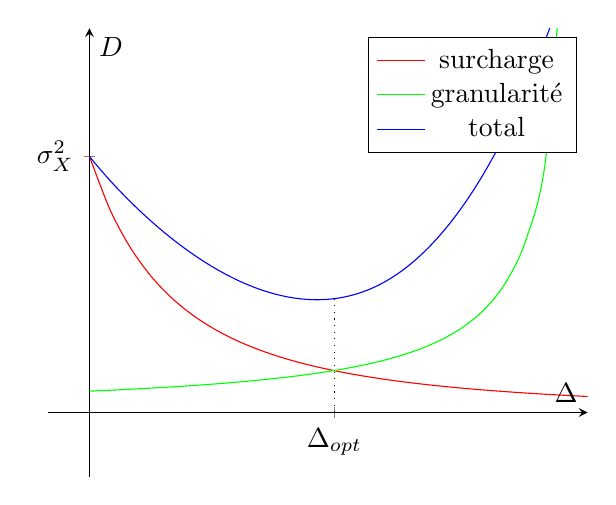
\begin{tikzpicture}
    \begin{axis}
      [axis lines=middle,
      xmin=-0.5, xmax=6,ymin=-0.5,ymax=3,
      xlabel=$\Delta$,ylabel=$D$,
      ytick={2},yticklabels={$\sigma_X^2$},
      xtick={2.95},xticklabels={$\Delta_{opt}$},
      domain=0:6]
      \addplot[red,smooth, no marks]{8/(x+2)^2};
      \addlegendentry{surcharge}
      \addplot[green,smooth, no marks]{1/(-x+6)};
      \addlegendentry{granularité}
      \addplot[blue,smooth,no marks,tension=1]coordinates{(0,2) (3.5,1) (6,4)};
      \addlegendentry{total}
      \addplot[dotted,black]coordinates{(2.95,0)(2.95,0.9)};
    \end{axis}
  \end{tikzpicture}
  \caption{Evolution de la distorsion en fonction du pas de quantification}
\end{figure}


\subsection{Quantification non uniforme}

On considère une source $X$ à valeur réelle $\mathcal{X} =\R$ décrite par une ddp $f_X(x)$. On chercje à quantifier cette source à l'aide d'un quantificateur non uniforme sur $M$ niveau décrit par:
\begin{itemize}
\item $M+1$ bornes des intervalles de quantification $b_0=\infty < b_1 < ... <b_M=+\infty$
\item $M$ valeurs de reconstruction $y_1 ... y_M$.
\end{itemize}
On choisit les paramètres de quantificateur de manière à minimiser une distorsion construite à partir d'une mesure quadratique.

Les conditions nécessaires pour avoir $D$ minimale sont :
\begin{itemize}
\item $\derivp[D]{y_i} = 0, \forall i=1\dots M$
\item $\derivp[D]{b_i} = 0, \forall i = 0\dots M$
\end{itemize}

\begin{align*}
\intertext{1ère condition d'optimalité}
\derivp[D]{y_i} & = \derivp{}{y_i} \int_{b_{i-1}}^{b_i} (x-y_i)^2 f_X(x) dx \\
& = - 2 \int_{b_{i-1}}^{b_i} (x-y_i) f_X(x) dx
\intertext{Ainsi,}
\derivp[D]{y_i} = 0 & \Leftrightarrow \int_{b_{i-1}}^{b_i} xf_X(x)dx = y_i \int_{b_{i-1}}^{b_i} f_X(x)dx \\
& \Rightarrow\boxed{ y_i = \frac{\int_{b_{i-1}}^{b_i} xf_X(x)dx}{\int_{b_{i-1}}^{b_i} f_X(x)dx}, \quad i = 1 \dots M}
\intertext{2ème condition d'optimalité}
\derivp[D]{b_i} & = \derivp{b_i} \int_{b_i}^{b_{i+1}} (x-y_{i+1})^2f_X(x)dx + \derivp{b_i}\int_{b_{i-1}}^{b_i} (x-y_i)^2 f_X(x)dx \\
& = -(b_i-y_{i+1})^2 f_X(b_i) + (b_i-y_i)^2 f_X(b_i)
\intertext{Ainsi, }
\derivp[D]{b_i} = 0 & \Leftrightarrow -(b_i-y_{i+1})^2 + (b_i-y_i)^2 = 0 \\
& \Leftrightarrow (y_{i+1}-y_i)(b_i-y_{i+1}+b_i-y_i) = 0 \\
& \Leftrightarrow \boxed{b_i = \frac{y_i+y_{i+1}}{2}, \quad i=1 \dots M-1}
\end{align*}
\begin{prop}
Les bornes des intervalles de quantification sont au milieu de deux valeurs de reconstructions consécutives.
\[
b_i = \frac{y_i+y_{i+1}}{2}, \quad i=1 \dots M-1
\]
et les valeurs de reconstructions optimales vérifient:
\[
  \hat{y_i}= E[\{X|X\in[b_i,b_{i+1}]\}] =  \frac{\displaystyle\int_{b_{i-1}}^{b_i} xf_X(x)dx}{\displaystyle\int_{b_{i-1}}^{b_i} f_X(x)dx}
\]


\end{prop}
\subsubsection{Algorithme de Lloyd -Max}
\begin{enumerate}
\item Initialisation : $b_0^{(0)} < b_1^{(0)} < \dots < b_n^{(0)}$ choisis arbitrairement, $k=1$.
\item $y_i^{(k)}$ obtenus à partir des $b_i^{(k-1)}, i=0 \dots M$ en utilisant la 1ère condition d'optimalité
\item $b_i^{(k)}$ obtenus à partir des $y_i^{(k)},i=1 \dots M$ en utilisant la 2ème condition d'optimalité
\item $k=k+1$
\item tant qu'il y a des variations des $y_i$ ou des $b_i$, aller en 2.
\end{enumerate}

\begin{rem}
Essayer d'implémenter l'algorithme de Lloyd-Max à l'aide de Matlab, C ou Python pour les fétichistes. Pour Matlab, utiliser la fonction \texttt{quad} afin de calculer les intégrales. Prendre une ddp gaussienne.

Essayer de retrouver ceci pour $M=4$ et $\sigma = 1$
\begin{center}
\begin{tabular}{ccc}
$i$ & $b_i$ & $y_i$ \\ \hline
1 & -0.98 & -1.51 \\
2 & 0 & -0.45 \\
3 & 0.98 & 0.45 \\
4 & $+\infty$ & 1.51 \\
\end{tabular}
\end{center}

Prendre l'infini égal à 10.
\end{rem}

\begin{rem}
On ne quantifie jamais sur le domaine des pixels, car les ddp y sont immondes. On effectue des transformées, et ensuite les ddp sont sympa (gaussiennes, laplaciennes), ce qui permet d'avoir des algorithmes efficaces.

La plupart du temps, les quantifications sont uniformes (JPEG, JPEG200, H264...). On n'utilise des quantifications non uniformes que dans le cas d'applications très précises, où le gain de 2 ou 3 dB sur le $RSB$ est vraiment nécessaire.
\end{rem}


\subsubsection{Comportement asymptotique}
Pour étudier le comportement asymptotique d'un quantificateur non uniforme, on suppose $M$ grand (les intervalles de quantification seront petits), $f_X(x) \approx f_X(y_i)$ sur $[b_{i-1},b_i]$. On note $\Delta_i = b_i - b_{i-1}$.\\

On a \[P_i = Pr(X\in[b_{i-1},b_i]) \approx f_X(y_i)\Delta_i\]

\begin{align*}
D & = \sum_{i=1}^M \int_{b_{i-1}}^{b_i} (x-y_i)^2 f_X(x) dx \\
D & = \sum_{i=1}^M f_X(y_i) \int_{b_{i-1}}^{b_i} (x-y_i)^2dx
\intertext{On suppose que $y_i$ est au milieu de l'intervalle $[b_{i-1},b_i]$}
\int_{b_{i-1}}^{b_i} (x-y_i)^2 dx & = \int_{-\Delta_i/2}^{\Delta_i/2} u^2 du = [\frac{u^3}{3}]_{-\Delta_i/2}^{\Delta_i/2} = \frac{2}{3} \frac{\Delta_i^2}{8} = \frac{\Delta_i^3}{12}
\intertext{En réinjectant dans $D$, on a}
D & = \sum_{i=1}^M f_X(y_i) \frac{\Delta_i^3}{12}
\intertext{On pose $\alpha_i^3  = f_X(y_i)\Delta_i^3$}
D & = \frac{1}{12} \sum_{i=1}^M \alpha_i^3
\intertext{Si on calcule}
\sum_{i=1}^M \alpha_i & = \sum_{i=1}^M (f_X(y_i))^{1/3} \Delta_i \approx \int_{-\infty}^{+\infty} (f_X(x))^{1/3} dx = cste
\intertext{On doit trouver les $\Delta_i$ et les $\alpha_i$ qui minimisent $D$ sous la contrainte $\sum_{i=1}^M \alpha_i = C$. On introduit donc le Lagrangien du problème :}
L(\alpha_1,\dots\alpha_M,\lambda) & = \frac{1}{12}\sum_{i=1}^M\alpha_i^3 + \lambda \left(\sum_{i=1}^M \alpha_i - C\right)
\intertext{Condition d'optimalité :}
\derivp[L]{\alpha_i} = 0 & \Rightarrow \frac{1}{4}\alpha_i^2 + \lambda = 0, \quad i = 1 \dots M \\
& \Rightarrow \alpha_i^2 = -4\lambda
\intertext{Les $\alpha_i$ sont donc tous égaux, d'où}
\alpha_i & = \frac{1}{M} \int_{-\infty}^{+\infty} (f_X(x))^{1/3} dx
\end{align*}
On avait $\alpha_i^3 = f_X(y_i) \Delta_i^3$. Ainsi, si $f_X(y_i)$ est grand, $\Delta_i$ est petit, et inversement.

%\img{0.5}{2/2/1}

On peut donc calculer la distorsion :
\begin{align*}
D & = \frac{1}{12} \sum_{i=1}^M \frac{1}{M^3}\left(\int_{-\infty}^{+\infty} (f_X(x))^{1/3}dx\right)^3 \\
& = \frac{1}{12} \left(\int_{-\infty}^{+\infty} (f_X(x))^{1/3}dx\right)^3.\frac{1}{M^2}
\intertext{Or, $M=2^R$ d'où}
D & = \frac{1}{12}\left(\int_{-\infty}^{+\infty} (f_X(x))^{1/3}dx\right)^3.2^{-2R}
\end{align*}

\begin{prop}
Comme pour la quantification uniforme, on a une décroissance en $2^{-2R}$ de la distorsion en fonction du débit. Ici, il y a un facteur multiplicatif qui dépend de la ddp de la source.

Pour une source quelconque de variance $\sigma_X^2$ le comportement débit / distorsion sera :
\[ \boxed{ D(R) = K \sigma_X^2 2^{-2R} \text{ avec } K = \frac{1}{12\sigma_X^2}(\int_{-\infty}^{+\infty} (f_X(x))^{1/3}dx)^3 } \]
Soit un rapport signal sur bruit:
\[
  RSB = \frac{\sigma_X^2}{D} = K . 2^{2R}
\]
\end{prop}

\begin{rem}
  Pour une source Gaussienne centrée on peux calculer $K$ et on a:
  \[
    D = \sigma^2 2^{-2R}
  \]
\end{rem}


\section{Quantification vectorielle}
\begin{defin}
  Un quantificateur vectoriel pour une source $\vec{X}\in\R^n$ est défini:

  \begin{itemize}
  \item par une fonction de quantification :
\[
  q : \R^n \to \{0, .... ,n-1\}
\]
\item par une fonction de reconstruction:
  \[
    q^{-1} :  \{0, .... ,n-1\} \to \R^n
  \]
  On note $\vec{y_m} = q^{-1}(m)$ les valeurs de reconstruction du quantificateur.
\end{itemize}
\end{defin}

On étend la notion de distorsion et de mesure de distorsion au cas vectoriel:

\begin{prop}[Mesure de distortion vectorielle]

  Mesure de distortion quadratique:\\
  \[
    d_2(\vec{x},\vec{y}) = \frac{1}{n}\sum_{i=1}^{n}|x_i-y_i|^2
  \]
  Mesure de distortion en valeur absolue:
  \[
    d_1(\vec{x},\vec{y})  = \frac{1}{n}\sum_{i=1}^{n}|x_i-y_i|
  \]
  La distorsion introduite par le quantificateur Q est alors l'espérance de la mesure de distorsion:
  \[
    D = E[d(\vec{x},Q(\vec{x}))]
  \]
\end{prop}
%\img{0.5}{2/2/2}

\subsection{Condition d'optimalité}

On considère une quantification vectorielle d'une source $\vec{X}\in\R^n$ sur $M$ niveau de quantification. On alors la distorsion:
\[
  D = \int_\R^n \|\vec{x}-Q(\vec{x})\|^2_2 f_{\vec{x}}(\vec{x})\d \vec{x}
\]

On partitionne $\R^n$ en cellule de quantification $\mathcal{C}^k, k\in[0...M-1]$ au seins desquelles  la valeur de reconstructio vaut $\vec{y_k}$.

\emph{Comment choisir $\mathcal{C}^k$ et $y_k$ pour minimiser $\vec{y_k}$?
}

\[
  D = \sum_{k=0}^{M-1}\int_{\mathcal{C}^k} \|\vec{x}-\vec{y_k}\|^2 f_\vec{X}(\vec{x})\d \vec{x}
\]
\begin{prop}

  Si on fixe les $\mathcal{C}^k$:

\[
  \vec{y_k} = \frac{\int_{\mathcal{C}^k}\vec{x}f_{\vec{X}}(\vec{x})\d\vec{x}}{\int_{\mathcal{C}^k}f_{\vec{X}}(\vec{x})\d\vec{x}}
\]


$  \vec{y_k}$ est le barycentre de $\mathcal{C}^k$ en utilisant la densité$f_{\vec{X}}(\vec{x})$.

Si on fixe les $\vec{y_k}$ alors pour minimiser $D$ il faut prendre:

\[
  \mathcal{C}^k =\{ \vec{x}\in\R^n ,\quad\|\vec{x}-\vec{y_k}\| \le \|\vec{x}-\vec{y_l}\| , \forall l \neq k\}
\]
\end{prop}
\begin{proof}

Si on suppose $\mathcal{C}^k$fixé alors pour fixer $y_k$ on calcule:
\[
  \derivp[D]{\vec{y_k}} = -2 \int_{\mathcal{C}^k} (\vec{x}-\vec{y_k})f_{\vec{X}}(x)\d\vec{x}
\]
On en déduit:

\[
  \vec{y_k} = \frac{\int_{\mathcal{C}^k}\vec{x}f_{\vec{X}}(\vec{x})\d\vec{x}}{\int_{\mathcal{C}^k}f_{\vec{X}}(\vec{x})\d\vec{x}}
\]
\end{proof}



 %%%%%%%%%%%%%%%%%%%%%%%%%%%%%%%%
Pour un couple (poids, taille), on peut :
\begin{itemize}
\item quantifier indépendamment le poids et la taille avec deux quantificateurs scalaires
\item les quantifier simultanément avec une quantification vectorielle
\end{itemize}

\subsection{Algorithme de Linde-Buzo-Gray}
\emph{Similaire à l'algorithme $K$-means}

\newcommand{\x}{\underline{x}}
Cet algorithme permet de fabriquer une quantification vectorielle optimale (optimum local) pour un ensemble de $K$ points de $\R^N$ : $\x_1 \dots \x_K$ et quantifiés sur $M$ niveaux.

\newcommand{\y}{\underline{y}}
Pour cela, on introduit la mesure de distorsion $d(\x,\y) = \frac{1}{N}||\x-\y||^2$.

Le quantificateur va minimiser la distorsion.\\

Initialisation :
\begin{itemize}
\item On sélectionne $M$ points $\y_1^{(0)},\dots,y_M^{(0)}$ parmi les $\x_1,\dots,\x_K$ au hasard.
\item $l=0, D_l = + \infty$
\end{itemize}

\begin{enumerate}
\item On réalise une quantification de $\x_1,\dots,\x_K$ en se servant de $\y_1^{(l)},\dots,\y_M^{(l)}$.
\[ q(\x_i) = \y_j \text{ ssi } ||\x_i-\y_j^{(l)}||^2 \leq ||\x_i-\y_k^{(l)}||^2, \quad \forall k\neq j\]

\newcommand{\Cc}{\mathcal{C}}

On obtient une partition de l'espace en cellules de quantification $\Cc_j^{(l)},j=1,\dots,M$ appelées cellules de Voronoï.

%\img{0.5}{2/3/1}

\item On calcule la distorsion :
\[ D^{(l+1)} = \frac{1}{K} \sum_{i=1}^K ||\x_i-q(\x_i)||^2 \]

\item Actualisation des valeurs de reconstruction. On considère l'ensemble des points appartenant à \[\Cc_j^{(l)} = \{ \x_1^{(l)},\dots, \x_{K_l}^{(l)} \}, \quad j = 1,\dots,M\]

On calcule le barycentre des points de $\Cc_j^{(l)}$ qui constitue la nouvelle valeur de reconstruction.

\[\y_j^{(l+1)} = \frac{1}{K_l} \sum_{i=1}^{K_l} \x_i^{(l)} \]

\item $l=l+1$

\item Aller en 1 tant que $D^{l-1} - D^l > \epsilon$

\end{enumerate}

L'algorithme LBG converge vers une minimum local de la distorsion.

\newcommand{\Cc}{\mathcal{C}}
En pratique :
\begin{itemize}
\item on transmet pour chaque $\x_i$ l'index $j$ de la cellule de Voronoi  $\Cc_j$ auquel il appartient.
\item il faut transmettre au récepteur l'ensemble des points de reconstruction $\y_1^{(\overline{l})},\dots,\y_M^{(\overline{l})}$ où $\overline{l}$ est l'index final des itérations.
\item la phase de réglage du quantificateur peut se faire sur seulement $L<<K$ points si on a beaucoup de points.
\end{itemize}
\section{Quantification scalable}
\emph{non traité en 2018-2019}
L'objectif est de permettre une flexibilité en terme de compression débit-distorsion. Une possibilité est d'avoir recours à un quantificateur scalable.\\

On considère une source uniforme sur $[-X_{max};X_{max}]$ quantifiée sur 8 niveaux.

%\img{0.5}{2/3/2}

Si on a $K$ échantillons à quantifier, on obtient $3K$ bits.\\

Les $K$ bits de poids fort sont placés dans un premier paquet.

Les $K$ bits de poids intermédiaire sont placés dans un second paquet.

Les $K$ bits de poids faible sont placés dans un troisième paquet.\\

Des utilisateurs disposant d'un mauvais canal recevront le premier paquet : la distorsion sera élevée.

Des utilisateurs disposant d'un excellent canal recevront les 3 paquets et auront une distorsion faible.\\

\begin{rem}
Cette méthode permet de réaliser une quantification sans avoir à connaître l'état du canal.
\end{rem}

\end{document}

%%% Local Variables:
%%% mode: latex
%%% TeX-master: "main"
%%% End:
